% ======================================================================
%  TFG Defense — Optical Music Recognition for Jazz Lead Sheets
%  Pol Casanovas Puig · FIB/UPC · June 2026
%  Compile:  latexmk -pdf defense.tex
% ======================================================================
\documentclass[aspectratio=169,11pt]{beamer}

% ── Theme ──────────────────────────────────────────────────────────────
\usetheme{Boadilla}
\useinnertheme{rounded}

% ── Colours: UPC identity ──────────────────────────────────────────────
\definecolor{upcblue}{RGB}{0,60,140}
\definecolor{upcbluelight}{RGB}{0,130,200}
\definecolor{upcgray}{RGB}{90,90,95}
\definecolor{metgreen}{RGB}{30,120,60}
\definecolor{metred}{RGB}{160,30,30}
\definecolor{metorange}{RGB}{180,90,0}

\setbeamercolor{structure}{fg=upcblue}
\setbeamercolor{frametitle}{bg=upcblue, fg=white}
\setbeamercolor{palette primary}{bg=upcblue, fg=white}
\setbeamercolor{palette secondary}{bg=upcblue!80, fg=white}
\setbeamercolor{palette tertiary}{bg=upcblue!60, fg=white}
\setbeamercolor{palette quaternary}{bg=upcblue!40, fg=white}
\setbeamercolor{block title}{bg=upcblue, fg=white}
\setbeamercolor{block body}{bg=upcblue!8, fg=black}
\setbeamercolor{alerted text}{fg=metred}
\setbeamercolor{example text}{fg=metgreen}

\setbeamerfont{frametitle}{size=\large, series=\bfseries}
\setbeamerfont{title}{size=\Large, series=\bfseries}
\setbeamerfont{block title}{series=\bfseries}

% ── Packages ───────────────────────────────────────────────────────────
\usepackage[T1]{fontenc}
\usepackage[utf8]{inputenc}
\usepackage{amsmath}
\usepackage{siunitx}
\usepackage{booktabs}
\usepackage{array}
\usepackage{tabularx}
\usepackage{graphicx}
\usepackage{tikz}
\usetikzlibrary{arrows.meta,positioning,shapes.geometric,calc,fit,backgrounds}

% Figures live two levels up in main/figures/
\graphicspath{
  {../main/figures/}
  {../main/figures/real_page/}
  {../main/figures/worst/}
}

% ── Navigation / footline ──────────────────────────────────────────────
\beamertemplatenavigationsymbolsempty
\setbeamertemplate{footline}{%
  \leavevmode
  \hbox{%
    \begin{beamercolorbox}[wd=0.34\paperwidth,ht=2.25ex,dp=1ex,center]{author in head/foot}%
      \usebeamerfont{author in head/foot}\insertshortauthor
    \end{beamercolorbox}%
    \begin{beamercolorbox}[wd=0.50\paperwidth,ht=2.25ex,dp=1ex,center]{title in head/foot}%
      \usebeamerfont{title in head/foot}\insertshorttitle
    \end{beamercolorbox}%
    \begin{beamercolorbox}[wd=0.16\paperwidth,ht=2.25ex,dp=1ex,right]{date in head/foot}%
      \usebeamerfont{date in head/foot}
      \insertframenumber{}/\inserttotalframenumber\hspace*{2ex}
    \end{beamercolorbox}%
  }%
}

% ── Shorthand macros ───────────────────────────────────────────────────
\newcommand{\metyes}{\textcolor{metgreen}{$\checkmark$}}
\newcommand{\metno}{\textcolor{metred}{$\times$}}
\newcommand{\metpart}{\textcolor{metorange}{$\circ$}}
\newcommand{\code}[1]{\texttt{\small #1}}

% ── Metadata ───────────────────────────────────────────────────────────
\title[OMR for Jazz Lead Sheets]{%
  End-to-End Optical Music Recognition\\
  for Jazz Lead Sheets}
\subtitle{Grau en Enginyeria Inform\`{a}tica (Computaci\'{o}) $\cdot$ TFG}
\author[Pol Casanovas Puig]{%
  Pol Casanovas Puig\\[3pt]
  {\small Supervisor: Manel Frigola Bourlon%
    \ (\emph{Dept.\ Automatic Control})}}
\institute[FIB / UPC]{%
  Facultat d'Inform\`{a}tica de Barcelona $\cdot$
  Universitat Polit\`{e}cnica de Catalunya}
\date{June 2026}

% ======================================================================
\begin{document}
% ======================================================================

% ── Title ─────────────────────────────────────────────────────────────
\begin{frame}[plain]
  \titlepage
\end{frame}

% ======================================================================
\section{Motivation}
% ======================================================================

\begin{frame}{A problem every jazz musician knows}
  \begin{columns}[T]
    \column{0.56\textwidth}
    \textbf{Years of jazz and big band experience\ldots}
    \medskip
    \begin{itemize}
      \item Rehearsals start, you get a stack of paper
      \item Brass section mixes concert-pitch and transposing instruments
        \begin{itemize}
          \item \textbf{B\(\flat\)} — trumpet, clarinet, soprano sax
          \item \textbf{E\(\flat\)} — alto sax, baritone sax
          \item \textbf{F} — French horn
        \end{itemize}
      \item You receive the lead sheet in one transposition, need it in another
      \item Manual on-paper transposition: slow, error-prone, and
            must be repeated every time
    \end{itemize}
    \medskip
    \alert{%
      \emph{The sheet music on this table is a real example.}\\[2pt]
      If it existed as structured data, transposition would be
      a single click.}
    \column{0.40\textwidth}
    \centering
    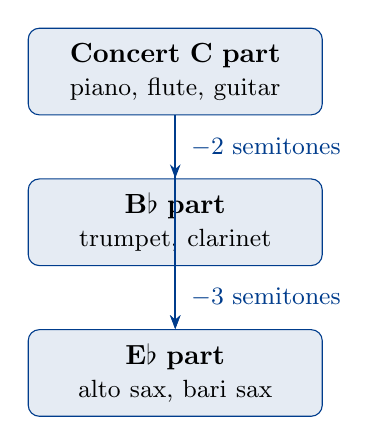
\begin{tikzpicture}
      \node[draw=upcblue,rounded corners,fill=upcblue!10,
            text width=3.5cm,align=center,minimum height=1.1cm] (c)
            {\textbf{Concert C part}\\{\small piano, flute, guitar}};
      \node[below=0.8cm of c,draw=upcblue,rounded corners,fill=upcblue!10,
            text width=3.5cm,align=center,minimum height=1.1cm] (bb)
            {\textbf{B\(\flat\) part}\\{\small trumpet, clarinet}};
      \node[below=0.8cm of bb,draw=upcblue,rounded corners,fill=upcblue!10,
            text width=3.5cm,align=center,minimum height=1.1cm] (eb)
            {\textbf{E\(\flat\) part}\\{\small alto sax, bari sax}};
      \draw[-{Stealth[length=5pt]},upcblue,thick] (c) -- (bb)
            node[midway,right=2pt,font=\small] {$-2$ semitones};
      \draw[-{Stealth[length=5pt]},upcblue,thick] (c) -- (eb)
            node[midway,right=2pt] {};
      \draw[-{Stealth[length=5pt]},upcblue,thick] (bb) -- (eb)
            node[midway,right=2pt,font=\small] {$-3$ semitones};
    \end{tikzpicture}
    \vspace{0.3cm}\\
    {\small Today: done by hand on paper.\\
    Goal: done automatically.}
  \end{columns}
\end{frame}

\begin{frame}{\textit{The Real Book} and the digitisation gap}
  \begin{columns}[T]
    \column{0.58\textwidth}
    \begin{itemize}
      \item Most widely circulated jazz fake book in the world
      \item Assembled by Berklee students in the 1970s; now officially published
      \item Hundreds of jazz standards --- on every musician's stand worldwide
      \item Official PDF is \textbf{image-only}: not searchable, not editable,
            not machine-readable
    \end{itemize}
    \medskip
    \textbf{What full digitisation would unlock:}
    \begin{itemize}
      \item \textbf{Automatic transposition} for all instrument families
      \item MIDI playback for practice
      \item Corpus-level harmonic analysis (jazz theory research)
      \item Search and catalogue for digital music libraries
    \end{itemize}
    \column{0.38\textwidth}
    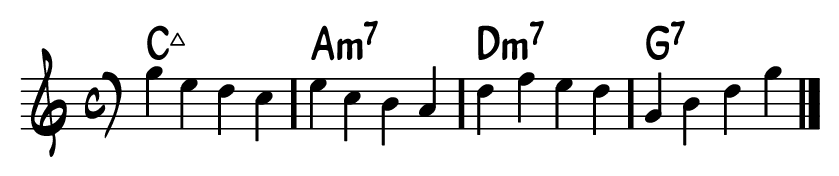
\includegraphics[width=\textwidth]{fig_leadsheet_excerpt}
    \vspace{0.1cm}\\
    {\small\centering
      Today: scan $\to$ image PDF\newline
      (no symbolic content)\par
      \vspace{0.3cm}
      \textbf{Goal:} scan $\to$ structured JSON\newline
      (pitch, rhythm, chords)}
  \end{columns}
\end{frame}

% ======================================================================
\section{Problem}
% ======================================================================

\begin{frame}{Four compounding challenges}
  \begin{columns}[T]
    \column{0.49\textwidth}
    \begin{block}{1. Notation complexity}
      Pitch = vertical position \emph{relative to the clef}.
      Duration = head shape + stem + flags + dots.
      Beams create joint dependencies across groups of notes.
      No standalone symbols.
    \end{block}
    \smallskip
    \begin{block}{3. Data scarcity}
      No publicly labelled corpus of Real Book pages.\\
      Must construct synthetic training data from scratch\\
      in the target engraving style.
    \end{block}
    \column{0.49\textwidth}
    \begin{block}{2. Domain gap}
      Models trained on clean computer-rendered images
      fail on real scans: noise, blur, perspective distortion,
      ink bleed, paper yellowing, JPEG artefacts.
    \end{block}
    \smallskip
    \begin{block}{4. Dual-stream recognition}
      A lead sheet carries two simultaneous streams:
      \textbf{melody} on the staff (pattern recognition)
      and \textbf{chord symbols} above it (character recognition).
      Existing OMR systems address only the first.
    \end{block}
  \end{columns}
\end{frame}

% ======================================================================
\section{System Design}
% ======================================================================

\begin{frame}{Five-stage inference pipeline}
  \centering
  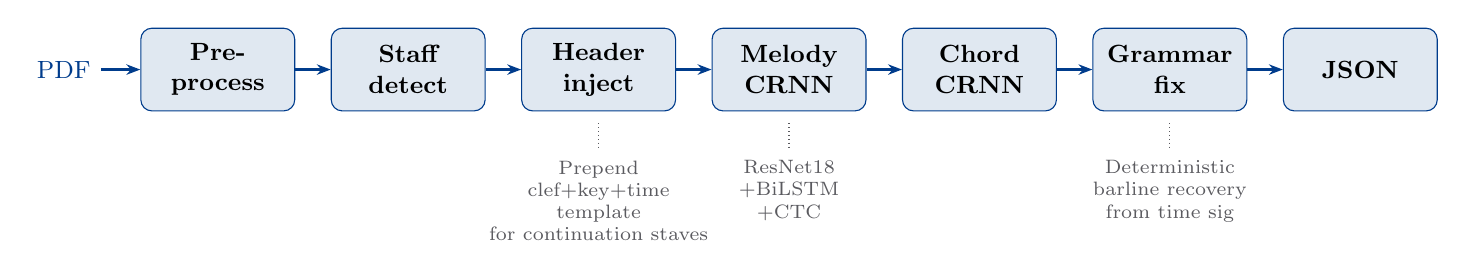
\begin{tikzpicture}[
    box/.style={draw=upcblue, rounded corners=4pt,
                fill=upcblue!12, text width=1.72cm, align=center,
                minimum height=1.05cm, font=\small\bfseries},
    dim/.style={draw=upcgray, rounded corners=3pt,
                fill=upcgray!10, text width=1.72cm, align=center,
                minimum height=0.85cm, font=\scriptsize},
    arr/.style={-{Stealth[length=5pt]}, upcblue, thick},
    note/.style={font=\scriptsize, text=upcgray, align=center}
  ]
    \node[box] (pre)   {Pre-\\process};
    \node[box, right=0.45cm of pre]  (det)  {Staff\\detect};
    \node[box, right=0.45cm of det]  (hdr)  {Header\\inject};
    \node[box, right=0.45cm of hdr]  (mel)  {Melody\\CRNN};
    \node[box, right=0.45cm of mel]  (crd)  {Chord\\CRNN};
    \node[box, right=0.45cm of crd]  (gfx)  {Grammar\\fix};
    \node[box, right=0.45cm of gfx]  (out)  {\textbf{JSON}};

    \draw[arr] ([xshift=-0.5cm]pre.west) -- (pre.west)
               node[pos=0, left, font=\small]{PDF};
    \foreach \a/\b in {pre/det, det/hdr, hdr/mel, mel/crd, crd/gfx, gfx/out}
      \draw[arr] (\a) -- (\b);

    % Annotations below
    \node[note, below=0.5cm of hdr, text width=2.8cm]
      {Prepend clef+key+time template\\for continuation staves};
    \node[note, below=0.5cm of mel, text width=1.9cm]
      {ResNet18\\+BiLSTM\\+CTC};
    \node[note, below=0.5cm of gfx, text width=2.4cm]
      {Deterministic barline recovery from time sig};

    \draw[densely dotted, upcgray]
      ([yshift=-0.15cm]hdr.south) -- ([yshift=0.05cm]hdr.south |- {$(hdr.south)+(0,-0.5cm)$});
    \draw[densely dotted, upcgray]
      ([yshift=-0.15cm]mel.south) -- ([yshift=0.05cm]mel.south |- {$(mel.south)+(0,-0.5cm)$});
    \draw[densely dotted, upcgray]
      ([yshift=-0.15cm]gfx.south) -- ([yshift=0.05cm]gfx.south |- {$(gfx.south)+(0,-0.5cm)$});
  \end{tikzpicture}

  \vspace{0.4cm}
  \begin{columns}[T]
    \column{0.32\textwidth}
    \small\textbf{Header injection (key design):}\\
    Continuation staves have no clef, key, or time signature.
    Injection keeps every staff in-distribution for the CRNN ---
    zero training cost, no leakage risk.
    \column{0.32\textwidth}
    \small\textbf{Two parallel CRNNs:}\\
    Separate model for each visual language.
    Melody: LMX token sequence.
    Chords: character-level recognition.
    \column{0.32\textwidth}
    \small\textbf{End-to-end latency:}\\
    \SI{114}{\milli\second} per page\\
    (8-staff page, RTX~3060, greedy decoding)
  \end{columns}
\end{frame}

\begin{frame}{Design decisions}
  \begin{columns}[T]
    \column{0.50\textwidth}
    \textbf{Why CRNN+CTC?}
    \smallskip

    \begin{tabular}{@{} l p{4.2cm} @{}}
      \toprule
      \textbf{Alternative} & \textbf{Reason rejected} \\
      \midrule
      Modular pipeline & Needs per-symbol segmentation labels (none available) \\[3pt]
      Seq2seq + attention & Adds encoder--decoder overhead with no benefit for left-to-right monophonic reading \\[3pt]
      Transformer (SMT, LEGATO) & State-of-the-art SER, but $>10\times$ compute; exceeds single-RTX-3060 budget \\
      \bottomrule
    \end{tabular}

    \smallskip
    \textbf{Backbone:} ResNet18 trains in half the time of VGG at comparable SER.

    \column{0.46\textwidth}
    \textbf{Why LMX?}
    \smallskip
    \begin{block}{\metno\ MusicXML}
      XML tree. Requires full hierarchical context to emit each node.
      Incompatible with CTC's atomic, left-to-right token stream.
    \end{block}
    \smallskip
    \begin{block}{\metyes\ LMX (chosen)}
      Flat, whitespace-delimited tokens.\\
      Each token is atomic: \code{pitch:C}, \code{quarter}, \code{flat}, \code{measure}.\\
      $\approx$100-token vocabulary.\\
      Regular grammar $\Rightarrow$ deterministic post-pass fixer.
    \end{block}
  \end{columns}
\end{frame}

% ======================================================================
\section{Data \& Training}
% ======================================================================

\begin{frame}{Synthetic data pipeline and quality control}
  \begin{columns}[T]
    \column{0.48\textwidth}
    \textbf{Building the training corpus:}
    \begin{itemize}
      \item PrIMuS: 87,678 monophonic incipits
      \item Re-rendered in \textbf{LilyJAZZ} style (matching Real Book typography)
      \item 3 domain filters $\Rightarrow$ 46,089 survive
      \item Split: 36,873 / 4,608 / 4,608 (train/val/test)
      \item Each sample: 1 clean + 2 scan-simulated PNGs
      \item $\approx$166,000 rendered assets on disk
    \end{itemize}
    \column{0.48\textwidth}
    \textbf{Scan simulation pipeline:}
    \begin{itemize}
      \item Gaussian + salt-and-pepper noise
      \item Motion blur and defocus
      \item Perspective distortion
      \item Ink bleed
      \item Paper yellowing (tone remap)
      \item JPEG compression
    \end{itemize}
    \medskip
    \textbf{Acceptance criterion:} clean-to-scanned SER gap $< 1$ pp.\\
    \textbf{Achieved:} $\Delta = \mathbf{0.06}$ pp.
  \end{columns}

  \vspace{0.25cm}
  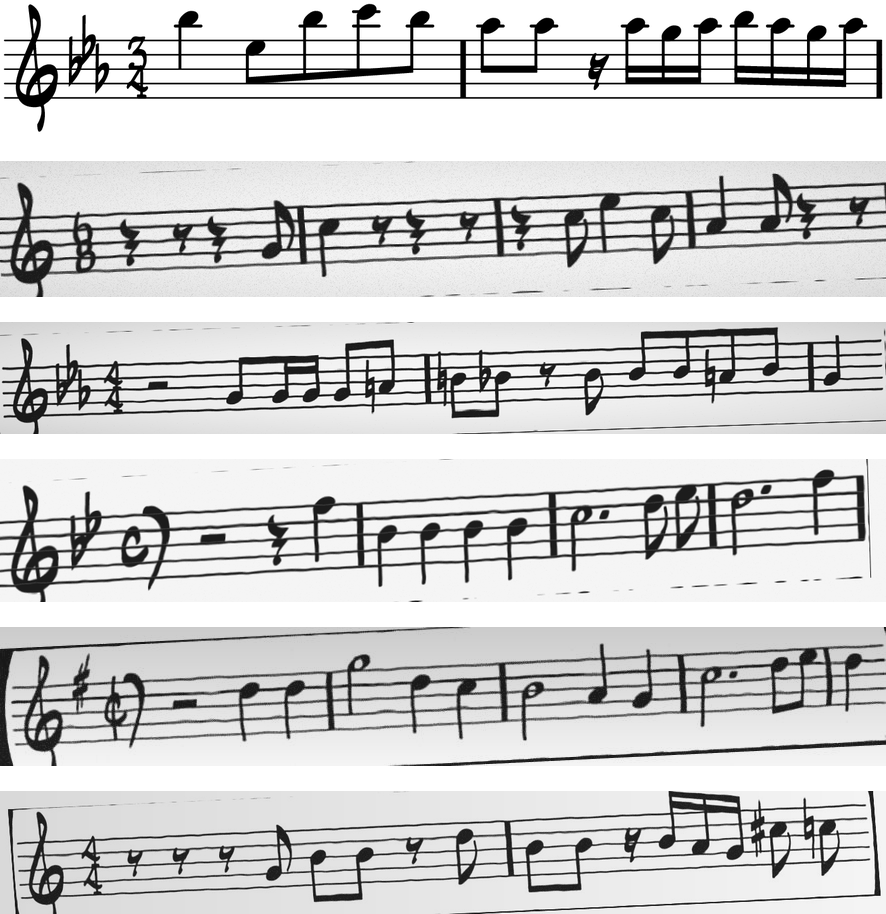
\includegraphics[width=\textwidth]{fig_augmentation_gallery}
\end{frame}

\begin{frame}{The twin leakage bug --- quality by finding the problem}
  \begin{columns}[T]
    \column{0.55\textwidth}
    \textbf{What happened:}
    \begin{enumerate}
      \item \code{extra\_data\_dirs} added derived image copies of training samples
      \item They joined the \emph{shared} split pool \textbf{before} the random permutation
      \item Near-duplicate training samples appeared in the val/test splits
      \item All metrics before 3 June 2026 were inflated
    \end{enumerate}
    \medskip
    \textbf{Fix applied:}
    \begin{itemize}
      \item Introduced \code{scanned\_variant\_dirs} --- train-only by construction, keyed by sample ID
      \item Clean split protocol re-run; all results in this presentation are post-fix
    \end{itemize}
    \column{0.41\textwidth}
    \begin{alertblock}{Why this is a positive outcome}
      Identifying data contamination mid-project, designing a leakage-safe mechanism,
      and re-reporting clean numbers is precisely the engineering rigour
      the project required.
      \medskip\\
      The metrics now reflect the true generalisation of the system.
    \end{alertblock}
  \end{columns}
\end{frame}

\begin{frame}{Training trajectory}
  \begin{columns}[T]
    \column{0.58\textwidth}
    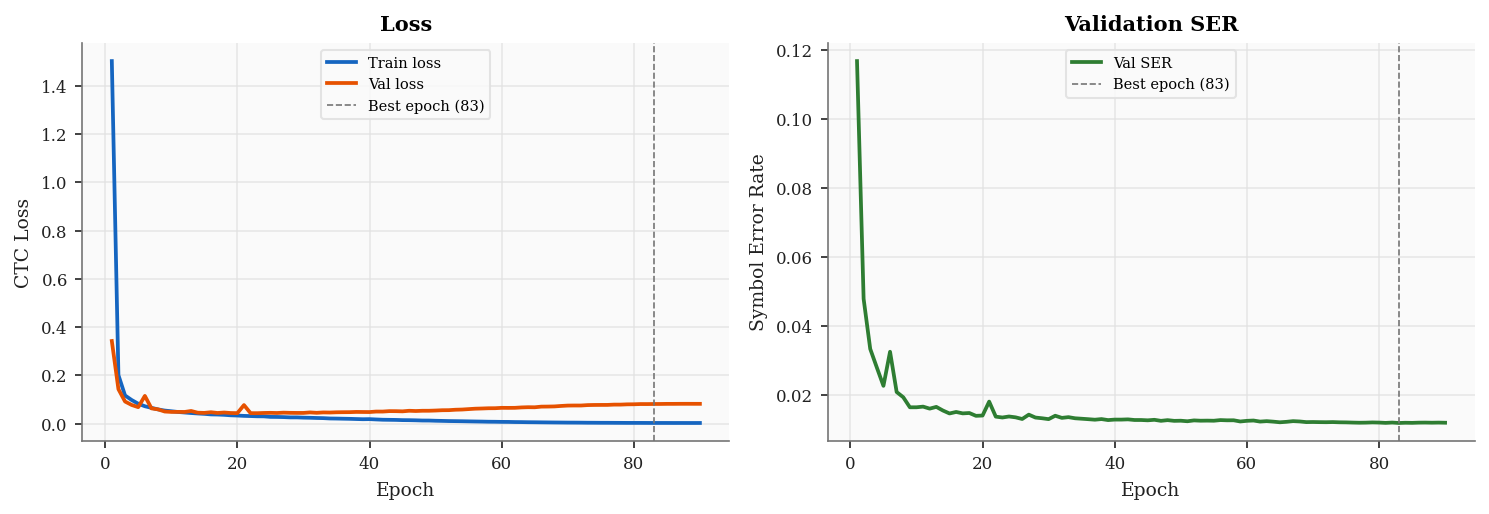
\includegraphics[width=\textwidth]{fig_training_curves}
    \column{0.38\textwidth}
    \textbf{Observations:}
    \begin{itemize}
      \item SER falls from $\approx\SI{12}{\percent}$ to $\approx\SI{2}{\percent}$
            by epoch~7 --- the alignment is learnt early
      \item Convergence to $\approx\SI{1.2}{\percent}$ by epoch~83
      \item Validation plateau: $\pm 0.02$ pp over last 10 epochs
      \item 90 epochs total, $\approx$13 h on RTX~3060
    \end{itemize}
    \medskip
    The training distribution is \textbf{scan-augmented only} --- clean images
    are held out for evaluation, so the gap is measured fairly.
  \end{columns}
\end{frame}

% ======================================================================
\section{Results}
% ======================================================================

\begin{frame}{Headline results}
  \centering
  \renewcommand{\arraystretch}{1.4}
  \begin{tabular}{@{} l
      S[table-format=2.2,
        table-number-alignment=right]
      S[table-format=2.2,
        table-number-alignment=right] @{}}
    \toprule
    \textbf{Metric}
      & {\textbf{Scanned (\%)}}
      & {\textbf{Clean (\%)}} \\
    \midrule
    Aggregate SER          & 1.23 & 1.17 \\
    Melodic SER            & 0.14 & 0.10 \\
    Perfect transcriptions & 72.7 & 73.7 \\
    SER $\le 5\%$          & 90.3 & 90.7 \\
    \bottomrule
  \end{tabular}

  \vspace{0.5cm}
  \begin{columns}[c]
    \column{0.30\textwidth}
    \centering
    \begin{block}{\metyes\ Target met}
      Scanned SER $1.23\% < 3\%$\\
      (target set at project start)
    \end{block}
    \column{0.34\textwidth}
    \centering
    \begin{block}{\metyes\ Melody is accurate}
      $\mathbf{99.86\%}$ of pitch, duration,\\
      and accidental tokens are correct
    \end{block}
    \column{0.30\textwidth}
    \centering
    \begin{block}{\metyes\ Gap is negligible}
      Clean vs scanned: $0.06$ pp\\
      (criterion: $< 1$ pp)
    \end{block}
  \end{columns}
\end{frame}

\begin{frame}{Error analysis --- where the residual error lives}
  \begin{columns}[T]
    \column{0.48\textwidth}
    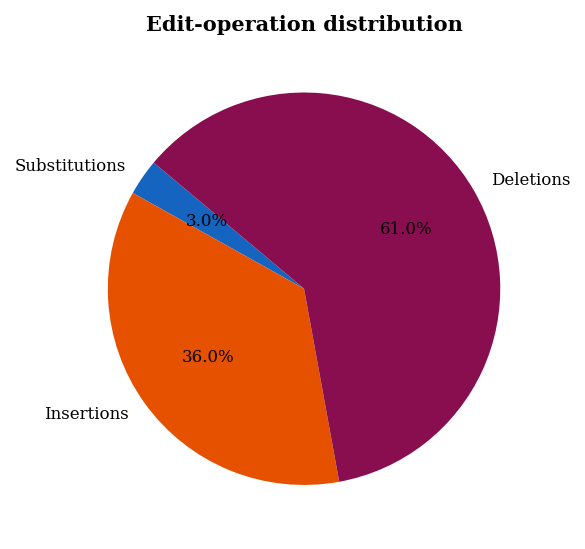
\includegraphics[width=\textwidth]{fig_error_pie}
    \column{0.48\textwidth}
    \textbf{3,506 total edits on the scanned split:}
    \begin{itemize}
      \item $\approx\mathbf{90\%}$ are \code{measure} (barline) and tie tokens
      \item Pitch and octave tokens barely appear in deletions or insertions
      \item Substitutions: only $3.4\%$ of all edits
    \end{itemize}
    \medskip
    \textbf{Most common substitution:}\\
    \code{pitch:B $\to$ pitch:G} (8 times over 4,608 staves)
    \medskip

    \begin{alertblock}{Key takeaway}
      The model reads the \textbf{music} correctly.
      It occasionally misplaces a \textbf{barline}.
      The melodic SER ($0.14\%$) measures this directly:
      once structural tokens are excluded, errors are negligible.
    \end{alertblock}
  \end{columns}
\end{frame}

\begin{frame}{\textit{Satin Doll} --- qualitative comparison}
  \begin{columns}[T]
    \column{0.48\textwidth}
    \centering
    \textbf{Audiveris 5.10 (state-of-the-art open-source)}
    \smallskip
    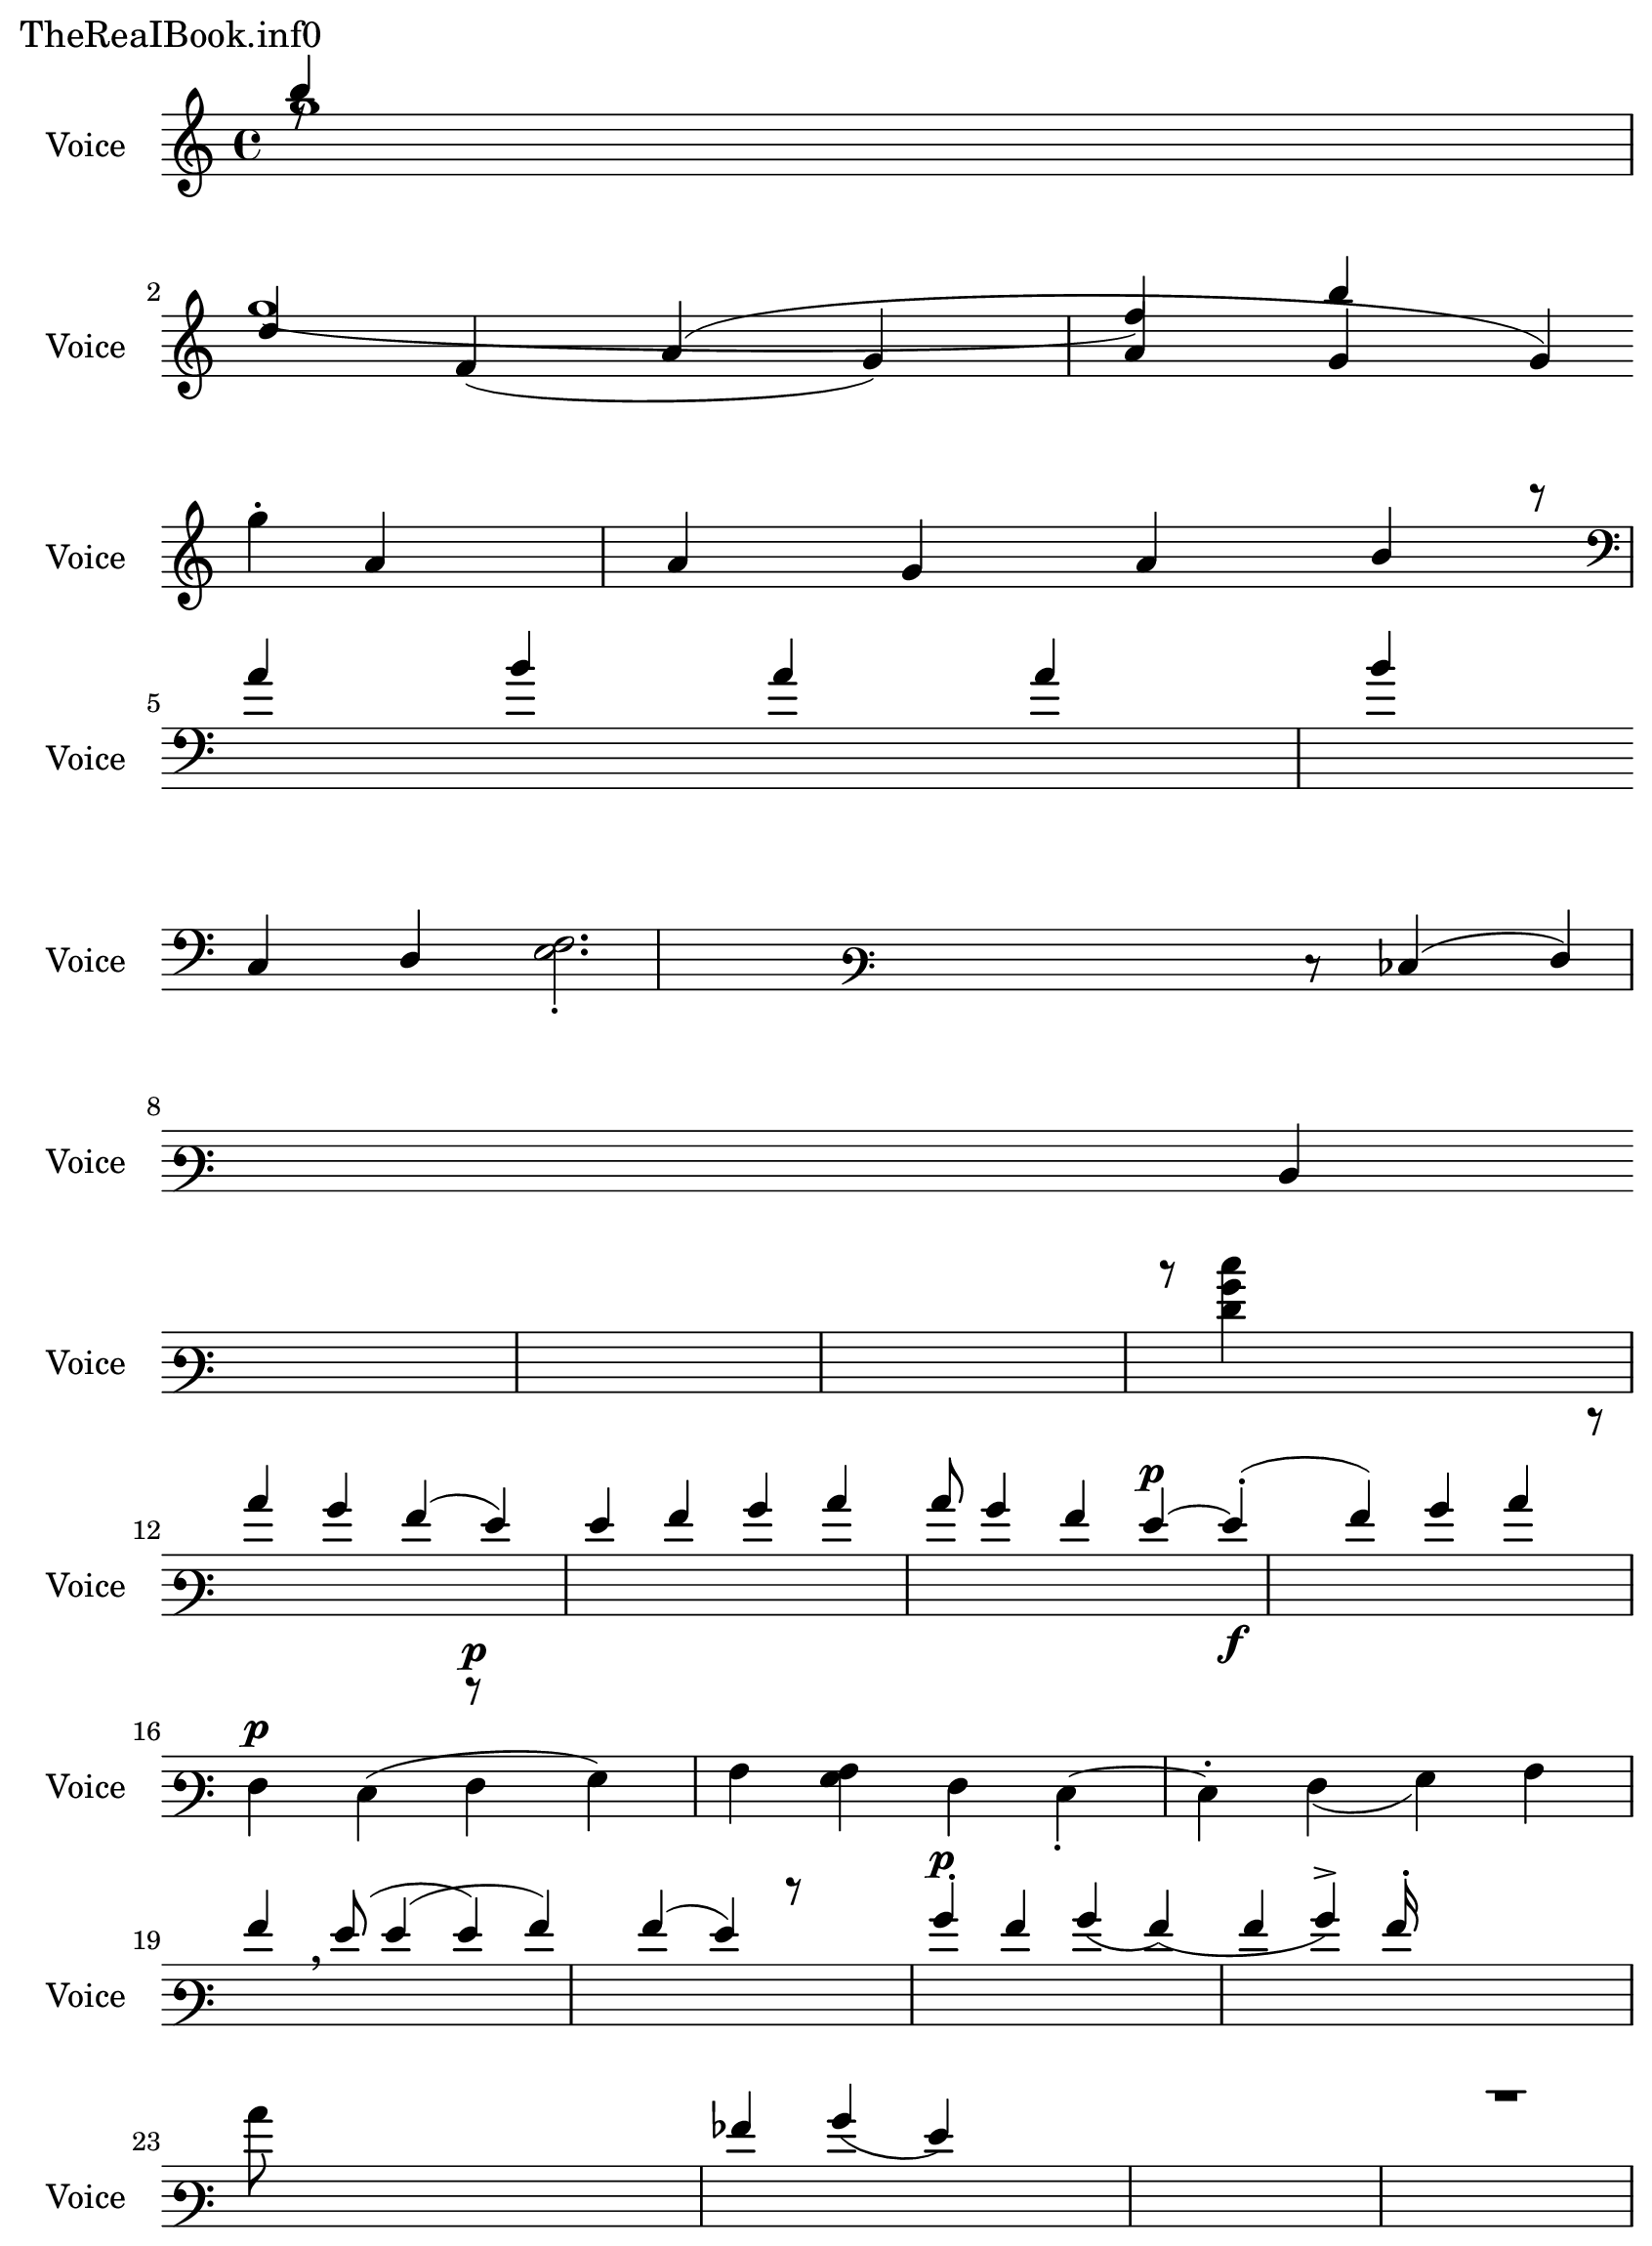
\includegraphics[width=\textwidth,height=4.2cm,keepaspectratio]{satin_audiveris}
    \smallskip
    \begin{itemize}
      \item[\metno] Correct clef on \textbf{2 of 9 staves}; rest default to bass clef
      \item[\metno] \textbf{No chord symbols} recovered
      \item[\metno] Octaves displaced; output musically unusable
    \end{itemize}
    \column{0.48\textwidth}
    \centering
    \textbf{This system}
    \smallskip
    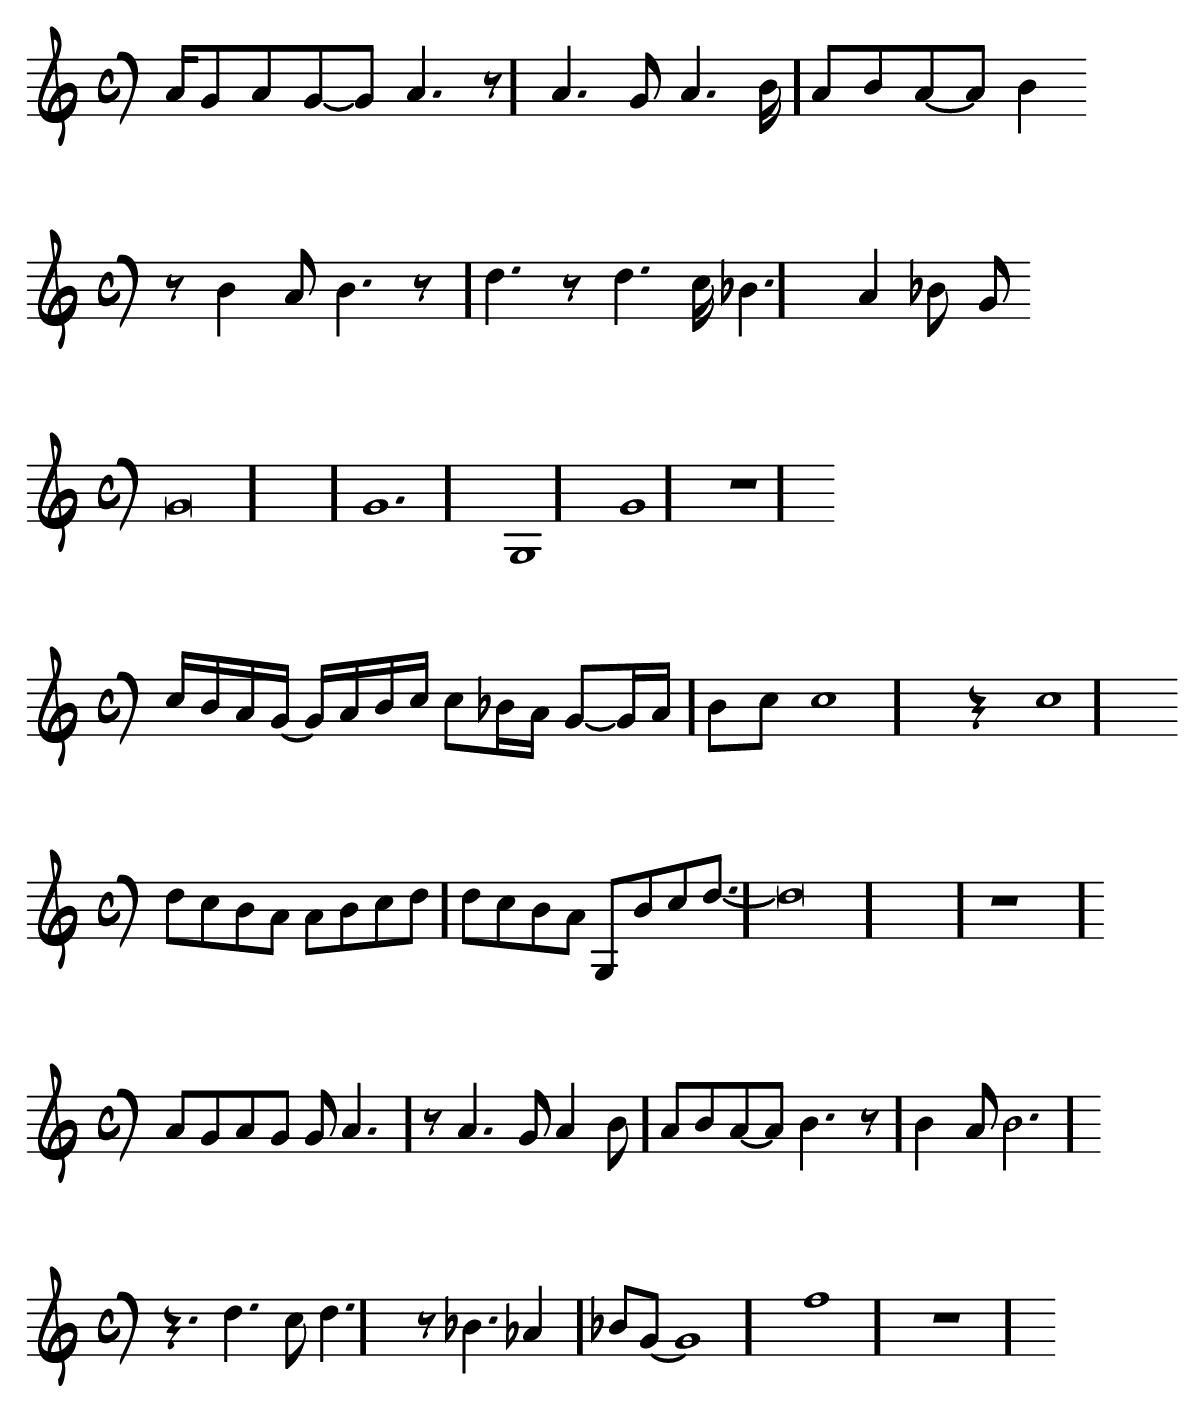
\includegraphics[width=\textwidth,height=4.2cm,keepaspectratio]{satin_ours_stacked}
    \smallskip
    \begin{itemize}
      \item[\metyes] \textbf{7 of 9 staves} recognised, all on correct treble clef
      \item[\metyes] \textbf{36 chord symbols} recovered:\\
            \code{D-7 G7 / E-7 A7 / G-7 C7 Fmaj7\,\ldots}
      \item[\metyes] Title band + credit line correctly rejected by gate
    \end{itemize}
  \end{columns}
\end{frame}

% ======================================================================
\section{Conclusions}
% ======================================================================

\begin{frame}{Work plan, sustainability, and adjustments}
  \begin{columns}[T]
    \column{0.50\textwidth}
    \textbf{Methodology:} incremental --- one pipeline stage at a time.\\
    \textbf{Budget:} 540 h (18 ECTS $\times$ 30 h/ECTS). On target.

    \medskip
    \textbf{Main deviation from plan:}
    \begin{itemize}
      \item Twin leakage discovery mid-project
      \item Response: redesign split protocol, introduce leakage-safe mechanism, re-train
      \item Added $\approx$2 weeks; resulted in clean, verifiable metrics
    \end{itemize}

    \column{0.46\textwidth}
    \textbf{Sustainability (Art.\ 12):}
    \begin{itemize}
      \item \textbf{Environmental:} $\approx$13 h GPU training, RTX~3060.
            Inference: 114 ms/page.
            No cloud compute, no distributed training.
      \item \textbf{Economic:} fully open-source stack (LilyPond, PyTorch, FastAPI).
            Zero licensing cost.
      \item \textbf{Social:} enables access to music archives.
            Dataset IP: PrIMuS (freely available);
            inference on The Real Book does not redistribute copyrighted content.
    \end{itemize}
  \end{columns}
\end{frame}

\begin{frame}{Objectives achieved}
  \renewcommand{\arraystretch}{1.3}
  \begin{tabular}{@{} c l @{}}
    \metyes & \textbf{General} --- SER $1.23\% < 3\%$ target on scan-simulated split \\
    \metyes & \textbf{O1} --- SoA survey; CRNN+CTC justified against three alternatives \\
    \metyes & \textbf{O2} --- Synthetic LilyJAZZ dataset from PrIMuS\\
            & \quad (46,089 samples; $\approx$166k rendered images) \\
    \metyes & \textbf{O3} --- Scan simulation; clean-to-scanned gap $= 0.06$ pp \\
    \metyes & \textbf{O4} --- CRNN+CTC: $1.17\%$ clean / $1.23\%$ scanned \\
    \metyes & \textbf{O5} --- Error analysis: $90\%$ structural tokens; pitch near-zero \\
    \metyes & \textbf{O6} --- Full inference pipeline + FastAPI + JSON output \\
    \metpart & \textbf{O7} --- Domain fine-tuning: 36 real staves, qualitative improvement; \\
             & \quad no held-out real SER (all 36 staves needed for training) \\
  \end{tabular}
\end{frame}

\begin{frame}{Conclusions and future work}
  \begin{columns}[T]
    \column{0.50\textwidth}
    \textbf{What was built and demonstrated:}
    \begin{itemize}
      \item End-to-end OMR system for jazz lead sheets
      \item $1.23\%$ aggregate SER on scan-simulated split
      \item $0.14\%$ melodic SER --- pitch is essentially error-free
      \item $72.7\%$ perfect transcriptions
      \item Chord recognition: $5.9\%$ CER after fine-tuning
            (from $69.9\%$ zero-shot)
      \item $114$ ms per page on RTX~3060
    \end{itemize}
    \column{0.46\textwidth}
    \textbf{Three concrete next steps:}
    \begin{enumerate}
      \item \textbf{Annotate $\geq$200 real staves} $\to$ held-out real-domain SER (binding constraint for O7)
      \item \textbf{Tuplet vocabulary} $\to$ largest single gap in LMX grammar coverage
      \item \textbf{Learned staff detector} (YOLO/DETR) $\to$ robustness on slanted and partial systems
    \end{enumerate}
  \end{columns}
  \medskip\hrule\medskip
  \textbf{Back to the original problem:}
  digitise \textit{The Real Book} $\to$ automatic transposition for
  B\(\flat\), E\(\flat\), and F instruments.
  This system makes that pipeline technically feasible.
\end{frame}

\begin{frame}{Technical competences (GEI / Computaci\'{o})}
  \begin{columns}[T]
    \column{0.48\textwidth}
    \begin{block}{CCO1.1 --- Algorithmic strategies \& performance}
      CRNN+CTC vs seq2seq vs transformer: justified on compute and data-efficiency grounds (\emph{Ch.\ 4}).\\
      Greedy vs beam search: $<0.01$ pp SER at $8\times$ cost --- greedy deployed (\emph{Ch.\ 6}).\\
      ResNet18 vs VGG: $2\times$ training time, comparable SER.\\
      Deterministic grammar fixer vs learned corrector.
    \end{block}
    \column{0.48\textwidth}
    \begin{block}{CCO2.4 --- Machine learning \& large data}
      CRNN+CTC supervised by CTC loss (\emph{Ch.\ 4--5}).\\
      $\approx$166,000 rendered training assets.\\
      Synthetic pre-training then domain fine-tuning applied to both CRNN streams.\\
      Data leakage discovered and remedied (\emph{Ch.\ 5}).
    \end{block}
  \end{columns}
  \vspace{0.3cm}
  Both competences declared \textbf{in depth} at TFG inscription.
\end{frame}

% ── Thank you / questions ─────────────────────────────────────────────
\begin{frame}[plain]
  \centering
  \vfill
  {\Huge\bfseries\color{upcblue} Thank you}\\[14pt]
  {\Large Questions?}\\[28pt]
  \hrule
  \vspace{14pt}
  \small
  \renewcommand{\arraystretch}{1.3}
  \begin{tabular}{@{} l l @{}}
    \textbf{SER}       & $1.23\%$ scanned / $1.17\%$ clean
                         (4,608 test samples, greedy CTC) \\
    \textbf{Melodic SER} & $0.14\%$ --- pitch content is essentially error-free \\
    \textbf{Perfect transcriptions} & $72.7\%$ \\
    \textbf{Chord CER} & $5.9\%$ after fine-tuning (from $69.9\%$ zero-shot) \\
    \textbf{Latency}   & $114$ ms/page on RTX~3060 \\[6pt]
    \textbf{Supervisor} & Manel Frigola Bourlon --- Dept.\ of Automatic Control \\
  \end{tabular}
  \vfill
\end{frame}

\end{document}
